
\begin{frame}
\frametitle{Computation of optimal loss $\mathcal L_{s, t}$
 for $s=3$ segments up to data point $t$}
  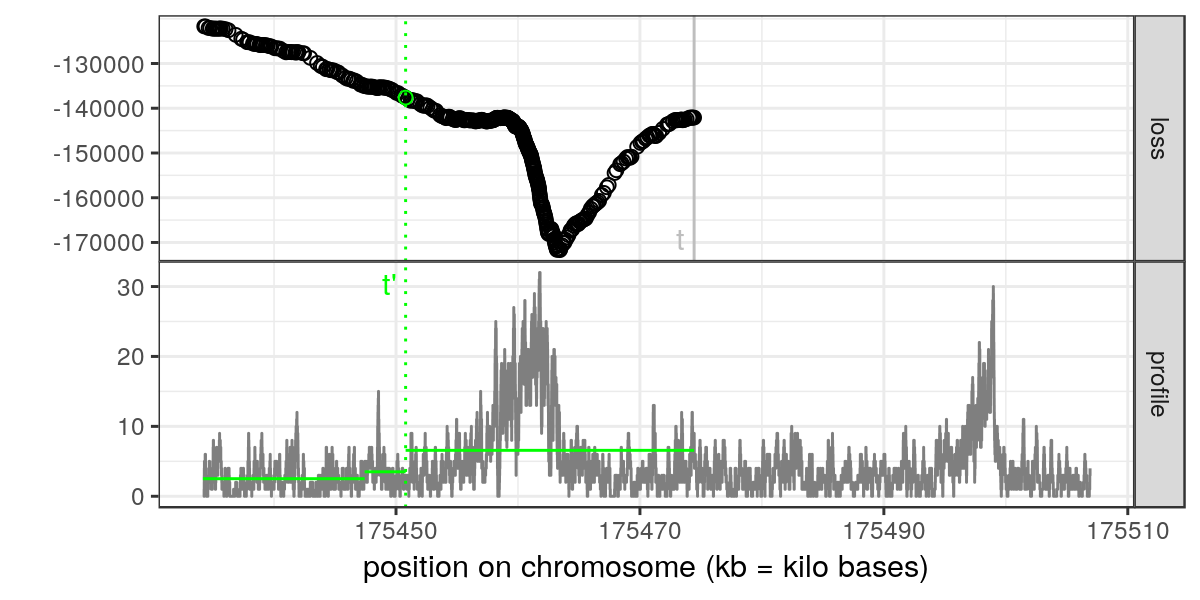
\includegraphics[width=\textwidth]{figure-dp-third-1.png}

$$
\mathcal L_{3, t} =
\min_{
  t' < t
}
\underbrace{
  \mathcal L_{2, t'}
}_{
  \text{optimal loss in 2 segments up to $t'$}
}
+
\underbrace{
  c_{(t', t]}
}_{
  \text{optimal loss of 3rd segment $(t', t]$}
}
$$

\end{frame}
 
\begin{frame}
\frametitle{Computation of optimal loss $\mathcal L_{s, t}$
 for $s=3$ segments up to data point $t$}
  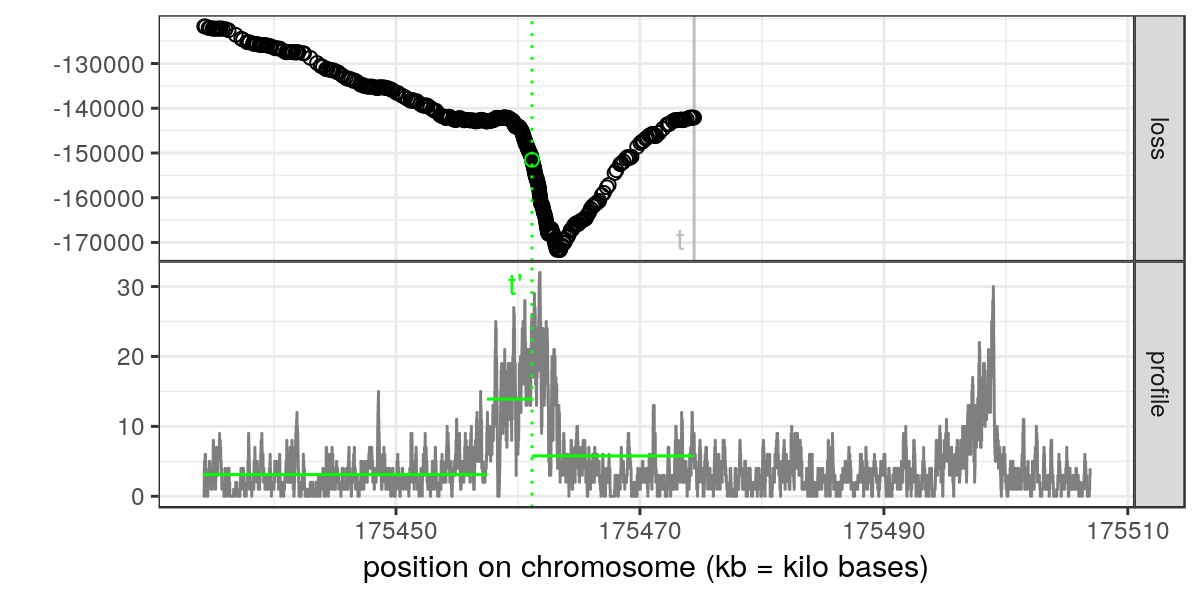
\includegraphics[width=\textwidth]{figure-dp-third-2.png}

$$
\mathcal L_{3, t} =
\min_{
  t' < t
}
\underbrace{
  \mathcal L_{2, t'}
}_{
  \text{optimal loss in 2 segments up to $t'$}
}
+
\underbrace{
  c_{(t', t]}
}_{
  \text{optimal loss of 3rd segment $(t', t]$}
}
$$

\end{frame}
 
\begin{frame}
\frametitle{Computation of optimal loss $\mathcal L_{s, t}$
 for $s=3$ segments up to data point $t$}
  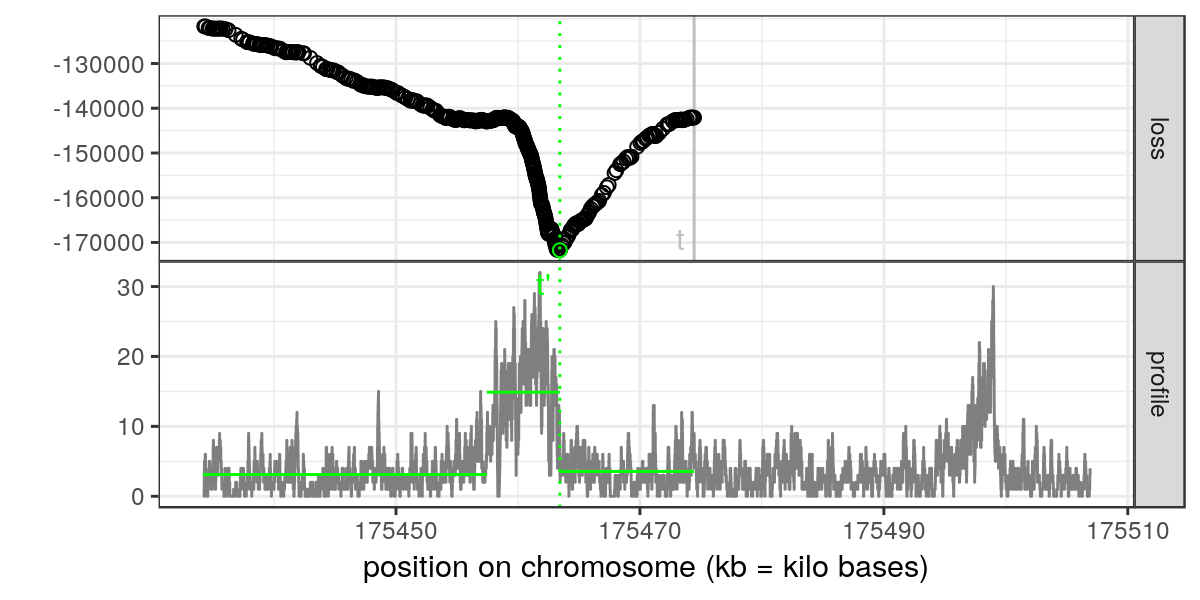
\includegraphics[width=\textwidth]{figure-dp-third-3.png}

$$
\mathcal L_{3, t} =
\min_{
  t' < t
}
\underbrace{
  \mathcal L_{2, t'}
}_{
  \text{optimal loss in 2 segments up to $t'$}
}
+
\underbrace{
  c_{(t', t]}
}_{
  \text{optimal loss of 3rd segment $(t', t]$}
}
$$

\end{frame}
 
\begin{frame}
\frametitle{Computation of optimal loss $\mathcal L_{s, t}$
 for $s=3$ segments up to data point $t$}
  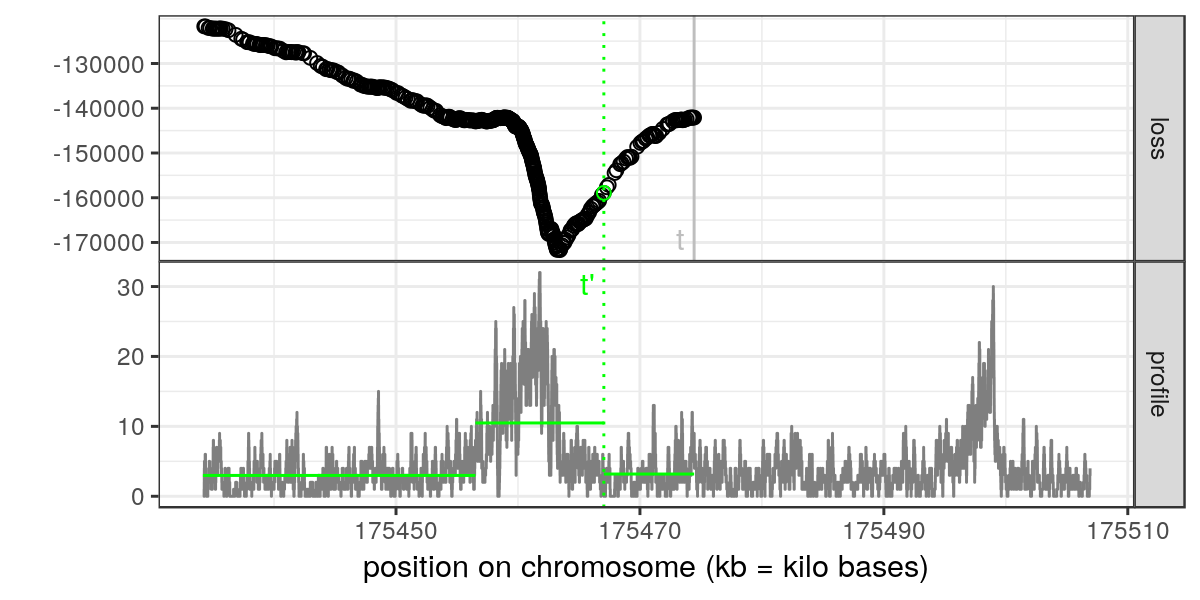
\includegraphics[width=\textwidth]{figure-dp-third-4.png}

$$
\mathcal L_{3, t} =
\min_{
  t' < t
}
\underbrace{
  \mathcal L_{2, t'}
}_{
  \text{optimal loss in 2 segments up to $t'$}
}
+
\underbrace{
  c_{(t', t]}
}_{
  \text{optimal loss of 3rd segment $(t', t]$}
}
$$

\end{frame}
